\documentclass{article}

% if you need to pass options to natbib, use, e.g.:
%     \PassOptionsToPackage{numbers, compress}{natbib}
% before loading neurips_2018

% ready for submission
%\usepackage{neurips_2018}

% to compile a preprint version, e.g., for submission to arXiv, add add the
% [preprint] option:
%     \usepackage[preprint]{neurips_2018}

% to compile a camera-ready version, add the [final] option, e.g.:
\usepackage[preprint, nonatbib]{neurips_2018}

% to avoid loading the natbib package, add option nonatbib:
%     \usepackage[nonatbib]{neurips_2018}

\usepackage[utf8]{inputenc} % allow utf-8 input
\usepackage[T1]{fontenc}    % use 8-bit T1 fonts
\usepackage{hyperref}       % hyperlinks
\usepackage{url}            % simple URL typesetting
\usepackage{booktabs}       % professional-quality tables
\usepackage{amsfonts}       % blackboard math symbols
\usepackage{amsmath}
\usepackage{graphicx,wrapfig,lipsum}
\usepackage{amsfonts}
\usepackage{booktabs}
\usepackage{empheq}
\usepackage{amsthm}
\usepackage{caption}
\usepackage{subcaption}
\usepackage{mathrsfs}  
\usepackage{amssymb}
\usepackage{tikz}
\usetikzlibrary{calc,positioning}

%\usepackage{nicefrac}       % compact symbols for 1/2, etc.
%\usepackage{microtype}      % microtypography
%\usepackage[title]{appendix}

\hyphenpenalty=10000

\theoremstyle{plain}
\newtheorem{thm}{Theorem}[section]
\newtheorem{proposition}[thm]{Proposition}
\newtheorem{lemma}[thm]{Lemma}
\newtheorem{corollary}[thm]{Corollary}

\theoremstyle{definition}
\newtheorem{definition}[thm]{Definition}
\newtheorem{remark}[thm]{Remark}
\newtheorem{example}[thm]{Example}

\newcommand{\nomath}[1]{\ifmmode
\mathrm{#1}%
\else
#1%
\fi}

\newcommand{\TODO}[1][]{\textcolor{red}{\ifx&#1&
\nomath{TODO}
\else
\nomath{TODO: #1}
\fi}}

% TODO: credit jeremy somewhere
% TODO: talk about how signatures are an easy way to impute, don't care about input length

\def\layersep{2.5cm}

\title{Deep Signatures}

\newlength{\imanol}
\settowidth{\imanol}{Imanol Perez Arribas}
\newcommand{\equallength}[1]{\makebox[\imanol][c]{#1}}

\author{ % alphabetical order
	\equallength{Patric Bonnier$^{1, }$\thanks{Equal contribution.}}
	\And
	\equallength{Patrick Kidger$^{1, 2, }$\footnotemark[1]}
	\And
	\equallength{Imanol Perez Arribas$^{1, 2, }$\footnotemark[1]}
	\And
	\equallength{Cristopher Salvi$^{1, 2, }$\footnotemark[1]}
	\And
	\equallength{Terry Lyons$^{1, 2}$}
	\AND \\[-12pt]
	\null$^1$ Mathematical Institute, University of Oxford \\
	\null$^2$ Alan Turing Institute \\
	\texttt{\{bonnier, kidger, perez, salvi, tlyons\}@\hspace{0.1pt}maths.ox.ac.uk}
}

\begin{document}
	\maketitle
	\begin{abstract}
		The signature of a stream of data is a collection of statistics known to provide an efficient description of the stream. It has previously been treated as a fixed feature transformation, on top of which a model may be built. But by mapping an input stream to a \emph{stream of streams} in a learnable way, and then applying the signature map stream-wise, we obtain a \emph{learned}, \emph{stream of signatures}. We emphasise both parts: not only are the terms of the signature selected in a learned way, but because the result is also a stream then the whole operation may be repeated arbitrarily many times. When the learnable map is a neural network then the operation of the signature may be interpreted as an activation function not operating element-wise; it is exploiting the stream-like nature of the data. In this manner signatures may be embedded as a layer anywhere within a neural network. We present the results of empirical experiments to back up the theoretical justification. Code available at \texttt{github.com/patrick-kidger/Deep-Signatures}.
	\end{abstract}
%	\TODO[more clickb8]
	\section{Introduction}
%	\TODO[I'd like to make subsection 1.1 shorter.]
% TODOs removed from pdf to help figure out the length
	%\subsection{Context} Is this needed?
	When data is ordered sequentially then it comes with a natural path-like structure: the data may be thought of as a discretisation of a path $X \colon [0, 1] \to V$, where $V$ is some Banach space. In practice we shall always take $V = \mathbb R^d$ for some $d \in \mathbb N$. For example the changing air pressure at a particular location may be thought of as a path in $\mathbb R$; the motion of a pen on paper may be thought of as a path in $ \mathbb R^2$; the changes within financial markets may be thought of as a path in $\mathbb R^d$, with $d$ potentially very large.
	
	Given a path, we may define its \emph{signature}, which is a collection of statistics of the path.
	
	\begin{definition}
		Let $\mathbf x = (x_1, \ldots, x_n)$, where $x_i \in \mathbb R^d$% for all $i = 1, 2, \ldots n $
		. Let $X \colon [0, 1] \to \mathbb R^d$ be continuous, such that $X_{(i -1) / (n - 1)} = x_i$, and linear on the intervals in between. Then letting $\otimes$ denote the tensor product, the signature of $\mathbf x$ is defined as the collection of iterated integrals
		\begin{align*}
		\mathrm{Sig}(\mathbf x) &= \left( \int_{0 < t_1 < \cdots < t_k < 1} \mathrm dX_{t_1} \otimes \cdots \otimes  \mathrm dX_{t_k} \right)_{k \geq 0} \\
		&= \left(\left( \int_{0 < t_1 < \cdots < t_k < 1} \mathrm dX^{i_1}_{t_1} \cdots \mathrm dX^{i_k}_{t_k} \right)_{1 \leq i_1, \ldots, i_k \leq d}\right)_{k\geq 0}.
		\end{align*}
	\end{definition}	
	We refer the reader to \cite{primer2016} for a primer on the use of the signature in machine learning. A brief overview of its key properties may be found in Appendix \ref{appendix:sigprop}. In short, the signature of a path determines the path essentially uniquely, and does so in an efficient, computable way. Furthermore, the signature is rich enough that every continuous function of the path may be approximated arbitrarily well by a linear function of its signature. Taken together these properties make the signature an attractive tool for machine learning. Most simply, the signature may be used as feature transformation, as it may often be simpler to learn a function of the signature than of the original path.
	
	Originally introduced and studied by Chen in \cite{Chen54, Chen57, Chen58}, the signature has seen use in finance \cite{TODO, TODO}, rough path theory \cite{lyons1998differential, FritzVictoir10} and machine learning \cite{yang2015chinese, xie2018learning, yang2016dropsample, yang2016deepwriterid, li2017lpsnet, yang2017leveraging, yang2016rotation, kiraly2016kernels, chevyrev2018signature}.
	
	The signature is an infinite sequence, so in practice some finite collection of terms must be selected. Since the magnitude of the terms exhibit factorial decay, see Appendix \ref{appendix:sigprop}, it is usual \cite{TODO} to simply choose the first $N$ terms of this sequence, which will typically be the largest terms. These first $N$ terms are called the \emph{truncated signature}, denoted $\mathrm{Sig}^N$. But if the function to be learned depended nontrivially on the higher degree terms, then crucial information has nonetheless been lost.
	
	This may be remedied. Apply a pointwise augmentation to the original stream of data before taking the signature. Then the first $N$ terms of the signature may better encode the necessary information \cite{kiraly2016kernels, chevyrev2018signature}. Explicitly, let $\Phi \colon \mathbb R^d \to \mathbb R^e$ be fixed; one could ensure that information is not lost by taking $\Phi(x) = (x, \varphi(x))$ for some $\varphi$. Then rather than taking the signature of $\mathbf x = (x_1, \ldots, x_n)$, where $x_i \in \mathbb R^d$, instead take the signature of $\Phi(\mathbf x) = (\Phi(x_1), \ldots, \Phi(x_n))$. In this way one may capture higher order information from the stream in the lower degree terms of the signature.
	
	\subsection{Our work}
	But how should this augmentation $\Phi$ be chosen? Previous work has fixed it arbitrarily, or experimented with several options before choosing one \cite{kiraly2016kernels, chevyrev2018signature}. Observe that in each case the map $\mathbf x \mapsto \mathrm{Sig}^N(\Phi(\mathbf x))$ is still ultimately just a feature transformation on top of which a model is learnt. Our more general approach is to allow the selection of $\Phi$ to be data-dependent, by having it be learnt; in particular it may be a neural network. Furthermore there is no reason it should necessarily operate pointwise, nor (since it is now learnt) need it be of the form $ (x, \varphi(x)) $. In this way we may enjoy the benefits of using signatures while avoiding their main limitation.
	
	But this means that the signature is essentially operating as a layer within a neural network. It consumes a tensor of shape $(b, d, s)$ -- corresponding to a batch of size $b$ of paths in $\mathbb R^d$ that have been sampled $s$ times -- and returns a tensor of shape $(b, (d^{N + 1} - 1)/(d - 1))$, where $N$ is the number of terms used in the truncated signature.\footnote{Observe that $(d^{N + 1} - 1)/(d - 1) = \sum_{k = 0}^N d^k$ is the number of scalar values in a signature with $N$ terms.} The signature is essentially an activation function that does not operate element-wise.
	
	There is no reason to stop here. If the signature layer works well once then it is natural to seek to use it again. The obvious problem is that the signature map consumes a stream of data and returns statistics which have no obvious stream-like qualities. The solution is to lift the input stream to a \emph{stream of streams}; for example, the stream of data $(x_1, \ldots, x_n)$ may be lifted to the `expanding snapshots' of $(\mathbf x_1, \ldots, \mathbf x_n)$, where $\mathbf x_i = (x_1, \ldots, x_i)$. Now apply the signature to each stream to obtain a stream of signatures $(\mathrm{Sig}^N(\mathbf x_1), \ldots, \mathrm{Sig}^N(\mathbf x_n))$, which is essentially a stream in Euclidean space. %This construction can be computed particularly efficiently, see \ref{re:efficiency}. % Trying to avoid references to specific parts of the appendix
	And now, on this new stream, we may augment it via a neural network and repeat the process again, as many times as we wish.
	
	In this way we arrive at the notion of \emph{deep signatures}.  % Important to have on a new line because of what we say about the name `deep signatures' later on.
	
	The remainder of the paper is laid out as follows. In Section 2 we briefly discuss some related work, in Section 3 we detail the specifics of embedding the signature as a layer within a neural network. Section 4, 5, 6, and 7 are dedicated to experiments; we demonstrate positive results in supervised learning problems, generative problems, and reinforcement learning problems.
	\section{Related Work}
	Some related work is by necessity already discussed in the introduction. We expand a little on their proposed models here.
	
	\begin{definition}
		The space of streams of data is defined as
		\begin{equation*}
		\mathcal S(\mathbb R^d) = \{ \mathbf x=(x_1, \ldots, x_n) : x_i \in \mathbb R^d, n \in \mathbb N\}.
		\end{equation*}
		Given $\mathbf x=(x_1, \ldots, x_n) \in \mathcal S(\mathbb R^d)$, the integer $n$ is called the length of $\mathbf x$.
	\end{definition}
	
	\begin{figure}
		\begin{subfigure}{\textwidth}
			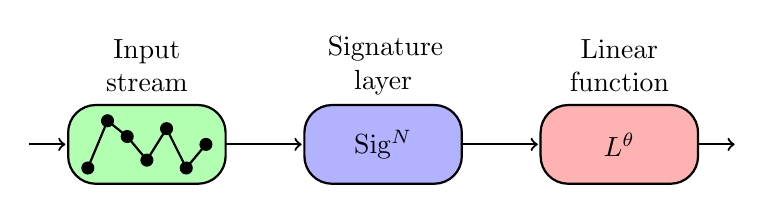
\begin{tikzpicture}[shorten >=1pt,draw=black!50, node distance=\layersep]
			
			\draw[black, thick, ->] (-0.5,0.5) -- (0,0.5);
			
			\draw[rounded corners=10pt, black, fill=green!30, thick]
			(0,0) rectangle ++(2,1);
			
			\draw[black, fill=black] (0.25,0.2) circle (.5ex);
			\draw[black, fill=black] (0.5,0.8) circle (.5ex);
			\draw[black, fill=black] (0.75,0.6) circle (.5ex);
			\draw[black, fill=black] (1,0.3) circle (.5ex);
			\draw[black, fill=black] (1.25,0.7) circle (.5ex);
			\draw[black, fill=black] (1.5,0.2) circle (.5ex);
			\draw[black, fill=black] (1.75,0.5) circle (.5ex);
			
			\draw[black, thick] (0.25,0.2) -- (0.5,0.8);
			\draw[black, thick] (0.5,0.8) -- (0.75,0.6);
			\draw[black, thick] (0.75,0.6) -- (1,0.3);
			\draw[black, thick] (1,0.3) -- (1.25,0.7);
			\draw[black, thick] (1.25,0.7) -- (1.5,0.2);
			\draw[black, thick] (1.5,0.2) -- (1.75,0.5);
			
			\node[text width=4em, text centered] at (1,1.5) {Input stream};
			
			\draw[rounded corners=10pt, black, fill=blue!30, thick]
			(3,0) rectangle ++(2,1);
			
			\node[text width=4em, text centered] at (4,1.5) {Signature layer};
			\node[text width=4em, text centered] at (4,0.5) {  Sig$ ^N $  };
			
			\draw[black, thick, ->] (2,0.5) -- (3,0.5);
			
			\draw[rounded corners=10pt, black, fill=red!30, thick]
			(6,0) rectangle ++(2,1);
			
			\node[text width=4em, text centered] at (7,1.5) {Linear function};
			\node[text width=6em, text centered] at (7,0.5) { $L^\theta$  };
			
			\draw[black, thick, ->] (5,0.5) -- (6,0.5);
			
			\draw[black, thick, ->] (8,0.5) -- (8.5,0.5);
			
			\end{tikzpicture}
			\centering
			\caption{Linear-signature model. Trainable parameters: $\theta$.}
			\label{fig:linear-sig}
		\end{subfigure}
		
		\begin{subfigure}{\textwidth}
			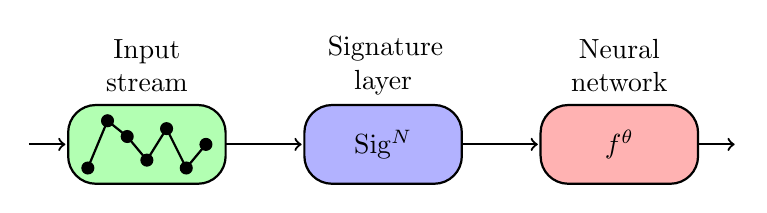
\begin{tikzpicture}[shorten >=1pt,draw=black!50, node distance=\layersep]
			
			\draw[black, thick, ->] (-0.5,0.5) -- (0,0.5);
			
			\draw[rounded corners=10pt, black, fill=green!30, thick]
			(0,0) rectangle ++(2,1);
			
			\draw[black, fill=black] (0.25,0.2) circle (.5ex);
			\draw[black, fill=black] (0.5,0.8) circle (.5ex);
			\draw[black, fill=black] (0.75,0.6) circle (.5ex);
			\draw[black, fill=black] (1,0.3) circle (.5ex);
			\draw[black, fill=black] (1.25,0.7) circle (.5ex);
			\draw[black, fill=black] (1.5,0.2) circle (.5ex);
			\draw[black, fill=black] (1.75,0.5) circle (.5ex);
			
			\draw[black, thick] (0.25,0.2) -- (0.5,0.8);
			\draw[black, thick] (0.5,0.8) -- (0.75,0.6);
			\draw[black, thick] (0.75,0.6) -- (1,0.3);
			\draw[black, thick] (1,0.3) -- (1.25,0.7);
			\draw[black, thick] (1.25,0.7) -- (1.5,0.2);
			\draw[black, thick] (1.5,0.2) -- (1.75,0.5);
			
			\node[text width=4em, text centered] at (1,1.5) {Input stream};
			
			\draw[rounded corners=10pt, black, fill=blue!30, thick]
			(3,0) rectangle ++(2,1);
			
			\node[text width=4em, text centered] at (4,1.5) {Signature layer};
			\node[text width=4em, text centered] at (4,0.5) {  Sig$ ^N $  };
			
			\draw[black, thick, ->] (2,0.5) -- (3,0.5);
			
			\draw[rounded corners=10pt, black, fill=red!30, thick]
			(6,0) rectangle ++(2,1);
			
			\node[text width=4em, text centered] at (7,1.5) {Neural network};
			\node[text width=6em, text centered] at (7,0.5) { $f^\theta$  };
			
			\draw[black, thick, ->] (5,0.5) -- (6,0.5);
			
			\draw[black, thick, ->] (8,0.5) -- (8.5,0.5);
			
			\end{tikzpicture}
			\centering
			\caption{Neural-signature model. Trainable parameters: $\theta$.}
			\label{fig:neural-sig}
		\end{subfigure}
		
		\begin{subfigure}{\textwidth}
			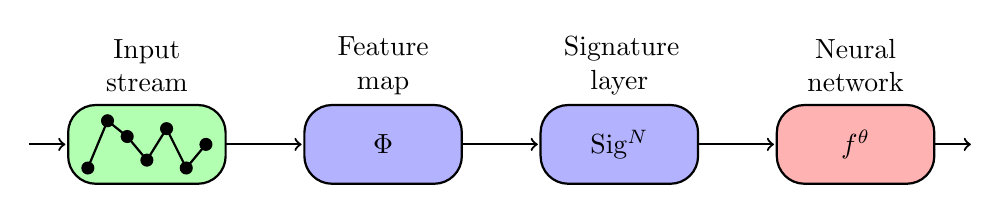
\begin{tikzpicture}[shorten >=1pt,draw=black!50, node distance=\layersep]
			
			\draw[black, thick, ->] (-0.5,0.5) -- (0,0.5);
			
			\draw[rounded corners=10pt, black, fill=green!30, thick]
			(0,0) rectangle ++(2,1);
			
			\draw[black, fill=black] (0.25,0.2) circle (.5ex);
			\draw[black, fill=black] (0.5,0.8) circle (.5ex);
			\draw[black, fill=black] (0.75,0.6) circle (.5ex);
			\draw[black, fill=black] (1,0.3) circle (.5ex);
			\draw[black, fill=black] (1.25,0.7) circle (.5ex);
			\draw[black, fill=black] (1.5,0.2) circle (.5ex);
			\draw[black, fill=black] (1.75,0.5) circle (.5ex);
			
			\draw[black, thick] (0.25,0.2) -- (0.5,0.8);
			\draw[black, thick] (0.5,0.8) -- (0.75,0.6);
			\draw[black, thick] (0.75,0.6) -- (1,0.3);
			\draw[black, thick] (1,0.3) -- (1.25,0.7);
			\draw[black, thick] (1.25,0.7) -- (1.5,0.2);
			\draw[black, thick] (1.5,0.2) -- (1.75,0.5);
			
			\node[text width=4em, text centered] at (1,1.5) {Input stream};
			
			\draw[rounded corners=10pt, black, fill=blue!30, thick]
			(3,0) rectangle ++(2,1);
			
			\node[text width=4em, text centered] at (4,1.5) {Feature map};
			\node[text width=4em, text centered] at (4,0.5) {  $\Phi$  };
			
			\draw[black, thick, ->] (2,0.5) -- (3,0.5);
			
			\draw[rounded corners=10pt, black, fill=blue!30, thick]
			(6,0) rectangle ++(2,1);
			
			\node[text width=4em, text centered] at (7,1.5) {Signature layer};
			\node[text width=4em, text centered] at (7,0.5) {  Sig$ ^N $  };
			
			\draw[black, thick, ->] (5,0.5) -- (6,0.5);
			
			\draw[rounded corners=10pt, black, fill=red!30, thick]
			(9,0) rectangle ++(2,1);
			
			\node[text width=4em, text centered] at (10,1.5) {Neural network};
			\node[text width=6em, text centered] at (10,0.5) { $ f^{\theta}$  };
			
			\draw[black, thick, ->] (8,0.5) -- (9,0.5);
			
			\draw[black, thick, ->] (11,0.5) -- (11.5,0.5);
			
			\end{tikzpicture}
			\centering
			\caption{Neural-signature-augment model. Trainable parameters: $\theta$.}
			\label{fig:neural-sig-aug}
		\end{subfigure}
		
		\caption{Three simple architectures with a signature layer.}
		\label{fig:simple-sig}
	\end{figure}
	
	Three simple models utilising the signature layer are shown in Figure \ref{fig:simple-sig}. In principle the universal approximation theorem for signatures (see Proposition \ref{prop:universal}) guarantees that the model shown in Figure \ref{fig:linear-sig} is rich enough to learn any continuous function. In practice, of course, the signature must be truncated, and it is not clear how to appropriately choose the truncation hyperparameter $N$.
	
	Thus a more practical approach is to replace the linear function on the signature by a nonlinear function, for example a neural network, see Figure \ref{fig:neural-sig}. This approach has been applied successfully in various tasks \cite{yang2015chinese, xie2018learning, yang2016dropsample, yang2016deepwriterid, li2017lpsnet, yang2017leveraging, yang2016rotation}.
	
	Following \cite{kiraly2016kernels, chevyrev2018signature}, one could also apply a pointwise transformation to the stream before the signature, lifting the $d$-dimensional stream of data $(x_1, \ldots, x_n) \in \mathcal S(\mathbb R^d)$ into a higher-dimensional feature space via a feature map $\Phi \colon \mathbb R^d \to \mathbb R^e$, yielding $(\Phi(x_1), \ldots, \Phi(x_n)) \in \mathcal S(\mathbb R^e)$. Then the signature of $\Phi(\mathbf x)$ may potentially capture properties of the stream of data that will make learning from data easier, see Figure \ref{fig:neural-sig-aug}.
	
	\section{The signature as a layer in a neural network}
	However, there is not always a clear candidate for the feature map $\Phi$ and a good choice might be very data-dependent. Thus we do the natural thing, and make $\Phi$ \emph{learnable} by taking $\Phi = \Phi^\theta$ to be a neural network with trainable parameters $\theta$. In this case, we again obtain the neural network shown in Figure \ref{fig:neural-sig-aug}, except that $\Phi$ is now also learnable.
	
	\subsection{Stream-preserving neural networks}
	
	% TODO: literally just quoting this from above and it's not great to repeat ourselves... but we need to state it somewhere outside the introduction too?!
	Recall that the signature consumes a tensor of shape $(b, d, s)$ -- corresponding to a batch of size $b$ of paths in $\mathbb R^d$ that have been sampled $s$ times -- and returns a tensor of shape $(b, (d^{N + 1} - 1)/(d - 1))$, where $N$ is the number of terms used in the truncated signature.
	
	Let $(x_1, \ldots, x_n) \in \mathcal S(\mathbb R^d)$ and $\Phi^\theta \colon \mathbb R^d \to \mathbb R^e$. Whatever the choice of $\Phi^\theta$, it must preserve the stream-like nature of the data if we are to take a signature afterwards. The simplest way of doing this is to have $\Phi^\theta$ operate pointwise:
	\begin{equation*}
	(\Phi^\theta(x_1), \ldots, \Phi^\theta(x_n)) \in \mathcal S(\mathbb R^e).
	\end{equation*}
	Another way to preserve the stream-like nature is to sweep a one dimensional convolution along the stream; more generally one could sweep a whole feedforward network along the stream. For some $ m \in \mathbb N $ this gives
	\begin{equation*}
	(\Phi^\theta(x_1, \ldots, x_m), \ldots, \Phi^\theta(x_{n - m + 1}, \ldots, x_n)) \in \mathcal S(\mathbb R^e).
	\end{equation*}
	More generally still, this could have memory, as in a recurrent neural network. Fix $m \in \mathbb N$, let $\Phi_{0} = 0$, and define $\Phi_k = \Phi^\theta\left(x_k, \ldots, x_{k + m}; \Phi_{k - 1}\right)$ for $k \in \{1, \ldots, n - m + 1\}$. Then
	\begin{equation*}
	(\Phi_1, \ldots, \Phi_{n -m +1}) \in \mathcal S(\mathbb R^e).
	\end{equation*}
	
	It is worth taking a moment to think what we really mean by `stream-like nature'. The signature map is defined on paths; it is applied to a stream of data in $\mathcal S(\mathbb R^d)$ by first interpolating the data into a path and then taking the signature. That is, the data is treated as a discretisation or set of observations of some underlying path.
	
	In principle one could reshape a tensor of shape $(b, ds)$ with no stream-like nature into one of shape $(b, d, s)$, and then take the signature. However it is not clear what this means mathematically: there is no underlying path which is being discretised. The signature is at this point an essentially arbitrary transformation, without the mathematical guarantees normally associated with it.
	
	\subsection{Backpropagation}
	At first glance the signature is not a pleasant-looking transformation. However despite being formed of integrals, the signature is in fact straightforward and efficient to compute, see Appendix \ref{appendix:sigprop}. More than that, the computation may in fact be described in terms of standard tensor operations. As such it may be backpropagated through without difficulty. % Mention Jeremy's thesis and a nicer way of calculating the backprop?
	
	In particular this means that having a learnable map before the signature does not pose a problem.
	
	\subsection{Multiple signature layers}	
	Now we would like not to restrict ourselves to a single signature layer. But as previously discussed, applying the signature layer `consumes' the stream-like nature of the data. The straightforward solution is to take a stream of signatures in the following way: given a stream $\mathbf x = (x_1, \ldots, x_n) \in \mathcal S(\mathbb R^d)$, let $\mathbf x_k = (x_1, \ldots, x_k)$ for $k=1, \ldots, n$, and apply the signature to each $\mathbf x_k$ to obtain the stream
	\begin{equation*}
	(\mathrm{Sig}^N(\mathbf x_1), \mathrm{Sig}^N(\mathbf x_2), \ldots, \mathrm{Sig}^N(\mathbf x_n)) \in \mathcal S(\mathbb R^{(d^{N + 1} - 1)/(d - 1)}).
	\end{equation*}
	Recall that the output of the signature is invariant to the length of the input stream.
	
	This notion may be generalised: let
	\begin{equation*}
	\ell = (\ell^1, \ell^2, \ldots, \ell^v) \colon \mathcal S(\mathbb R^d) \to \mathcal S(\mathcal S(\mathbb R^e)) \in \mathcal S(\mathbb R^{(e^{N + 1} - 1)/(e - 1)}),
	\end{equation*}
	which we refer to as a lift into the space of streams of streams.\footnote{And $v$ will likely depend on the length of the input to $\ell$.} Then we apply the signature stream-wise to obtain
	\begin{equation*}
	\mathrm{Sig}^N(\ell(\mathbf x)) = \left(\mathrm{Sig}^N(\ell^1(\mathbf x)), \ldots, \mathrm{Sig}^N(\ell^v(\mathbf x))\right).
	\end{equation*}
	In the above example, $\ell(\mathbf x) = (\mathbf x_1, \ldots, \mathbf x_n)$. Other plausible choices are to cut up $\mathbf x$ into multiple pieces, for example
	\begin{equation*}
	\ell(\mathbf x) = ((x_1, x_2), (x_3, x_4), \ldots, (x_{2\lfloor n/2 \rfloor - 1}, x_{2\lfloor n/2 \rfloor})),
	\end{equation*}
	or to take a sliding window
	\begin{equation*}
	\ell(\mathbf x) = ((x_1, x_2, x_3), (x_2, x_3, x_4), \ldots, (x_{n - 2}, x_{n - 1}, x_n)).
	\end{equation*}
	
	And now we may repeat the whole process as many times as desired; see Figure \ref{fig:deep signatures}. This defines the \emph{deep signature model}. The name comes from the fact that the signature is now embedded deep within the network instead of operating as a feature transformation. When there are multiple signature layers in a network, so that signatures-of-signatures are computed, then the name may be taken to have a double meaning, but we stress that this need not be the case. Good results may often be obtained with only a single signature layer.  % So I think this bit is quite important... it makes the name `deep signatures' suitable even for single-sig models.
	
	\begin{figure}
		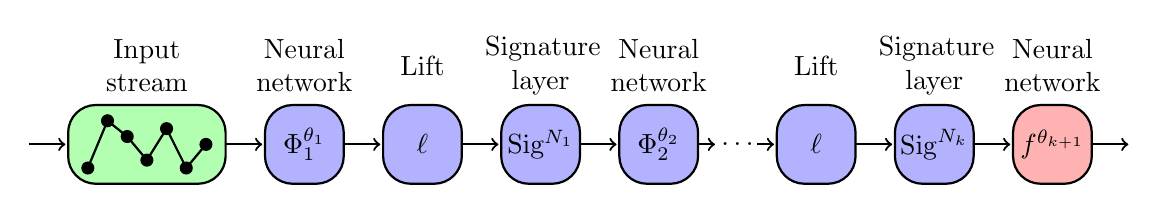
\begin{tikzpicture}[shorten >=1pt,draw=black!50, node distance=\layersep]
		
		\draw[black, thick, ->] (-0.5,0.5) -- (0,0.5);
		
		\draw[rounded corners=10pt, black, fill=green!30, thick]
		(0,0) rectangle ++(2,1);
		\draw[black, fill=black] (0.25,0.2) circle (.5ex);
		\draw[black, fill=black] (0.5,0.8) circle (.5ex);
		\draw[black, fill=black] (0.75,0.6) circle (.5ex);
		\draw[black, fill=black] (1,0.3) circle (.5ex);
		\draw[black, fill=black] (1.25,0.7) circle (.5ex);
		\draw[black, fill=black] (1.5,0.2) circle (.5ex);
		\draw[black, fill=black] (1.75,0.5) circle (.5ex);
		\draw[black, thick] (0.25,0.2) -- (0.5,0.8);
		\draw[black, thick] (0.5,0.8) -- (0.75,0.6);
		\draw[black, thick] (0.75,0.6) -- (1,0.3);
		\draw[black, thick] (1,0.3) -- (1.25,0.7);
		\draw[black, thick] (1.25,0.7) -- (1.5,0.2);
		\draw[black, thick] (1.5,0.2) -- (1.75,0.5);
		\node[text width=4em, text centered] at (1,1.5) {Input stream};
		
		\draw[black, thick, ->] (2,0.5) -- (2.5,0.5);
		
		\draw[rounded corners=10pt, black, fill=blue!30, thick]
		(2.5,0) rectangle ++(1,1);		
		\node[text width=4em, text centered] at (3,1.5) {Neural network};
		\node[text width=4em, text centered] at (3,0.5) {  $ \Phi_1^{\theta_1} $  };
		
		\draw[black, thick, ->] (3.5,0.5) -- (4,0.5);
		
		\draw[rounded corners=10pt, black, fill=blue!30, thick]
		(4,0) rectangle ++(1,1);
		\node[text width=4em, text centered] at (4.5,1.5) {Lift};
		\node[text width=4em, text centered] at (4.5,0.5) {  $\ell$  };
		
		\draw[black, thick, ->] (5,0.5) -- (5.5,0.5);
		
		\draw[rounded corners=10pt, black, fill=blue!30, thick]
		(5.5,0) rectangle ++(1,1);
		\node[text width=4em, text centered] at (6,1.5) {Signature layer};
		\node[text width=4em, text centered] at (6,0.5) {  Sig$ ^{N_1} $  };
		
		\draw[black, thick, ->] (6.5,0.5) -- (7,0.5);
		
		\draw[rounded corners=10pt, black, fill=blue!30, thick]
		(7,0) rectangle ++(1,1);
		\node[text width=4em, text centered] at (7.5,1.5) {Neural network};
		\node[text width=4em, text centered] at (7.5,0.5) {$\Phi_2^{\theta_2}$};
		
		\draw[black, thick, ->] (8,0.5) -- (8.25,0.5);
		
		\node[text width=4em, text centered] at (8.5,0.5) {$\ldots$};	
		
		\draw[black, thick, ->] (8.75,0.5) -- (9,0.5);
		
		\draw[rounded corners=10pt, black, fill=blue!30, thick]
		(9,0) rectangle ++(1,1);
		\node[text width=4em, text centered] at (9.5,1.5) {Lift};
		\node[text width=4em, text centered] at (9.5,0.5) {$\ell$};
		
		\draw[black, thick, ->] (10,0.5) -- (10.5,0.5);
		
		\draw[rounded corners=10pt, black, fill=blue!30, thick]
		(10.5,0) rectangle ++(1,1);
		\node[text width=4em, text centered] at (11,1.5) {Signature layer};
		\node[text width=4em, text centered] at (11,0.5) {$\mathrm{Sig}^{N_k}$};
		
		\draw[black, thick, ->] (11.5,0.5) -- (12,0.5);
		
		\draw[rounded corners=10pt, black, fill=red!30, thick]
		(12,0) rectangle ++(1,1);
		\node[text width=4em, text centered] at (12.5,1.5) {Neural network};
		\node[text width=4em, text centered] at (12.5,0.5) {$f^{\theta_{k+1}}$};
		
		\draw[black, thick, ->] (13,0.5) -- (13.5,0.5);
		
		
		\end{tikzpicture}
		\centering
		\caption{Deep signature model. Trainable parameters: $\theta_1, \ldots, \theta_{k + 1}$.}
		\label{fig:deep signatures}
	\end{figure}
	
\section{Supervised learning with fractional Brownian motion}

 % TODO: change shape of this plot. Fix TeX overlay.
\begin{wrapfigure}{r}{0.5\textwidth}
	\resizebox{\linewidth}{!}{%
		\begin{tikzpicture}
			\node at (0, 0){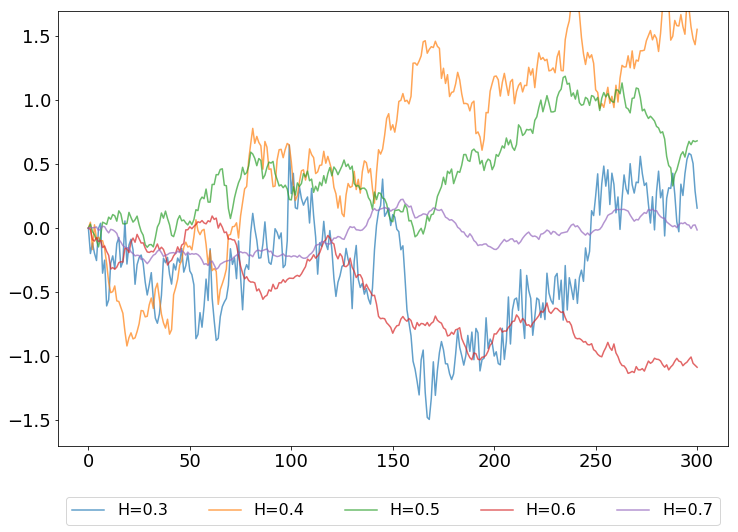
\includegraphics[width=30em]{figures/simulation}};
			\node at (0.3, -3.2){$t$};
			\node at (-5.2, 0.3){$B^H_t$};
		\end{tikzpicture}
	}
	\captionsetup{width=0.9\linewidth}
	\caption{Realisations of fractional Brownian motion with different Hurst parameters.}
	\label{fig:simulation}
\end{wrapfigure} 

Fractional Brownian motion \cite{mishura2008stochastic} is a Gaussian process $B^H \colon [0,\infty) \rightarrow \mathbb{R}$ that generalises Brownian motion. It is self-similar and exhibits fractal-like behaviour. Unlike classical Brownian motion, increments of fractional Brownian motion need not be independent. Fractional Brownian motion depends upon a parameter $H \in (0, 1)$, known as the Hurst parameter. Examples are shown in Figure \ref{fig:simulation}; note how lower Hurst parameters result in noticeably rougher paths.

Fractional Brownian motion has been successfully used to model phenomena in diverse fields. For example, empirical evidence from financial markets \cite{gatheral2014volatility} suggests that log-volatility is well modelled by fractional Brownian motion with Hurst parameter $H \approx 0.1$. The case of $H = \frac{1}{2}$ corresponds to usual Brownian motion.  % TODO: fit in somewhere: 

Estimating the Hurst parameter of a fractional Brownian motion path is considered a challenging task because of the paths' non-stationarity and long range dependencies \cite{lacasa2009visibility}. We train a variety of models to perform this estimation. That is, to learn the map
\begin{equation*}
\mathbf x^H \mapsto H,
\end{equation*}
where $\mathbf x^H = ((t_0, x_0), (t_1, x_1), \ldots, (t_n, x_n)) \in \mathcal S(\mathbb R^2)$ with $x_i= B^H_{t_i}$ for some realisation of $B^H$.

The results are shown in Figures \ref{fig:fbm results} and \ref{fig:fbm comparison}.

\begin{figure}
	\begin{subfigure}{0.5\textwidth}
			\centering
			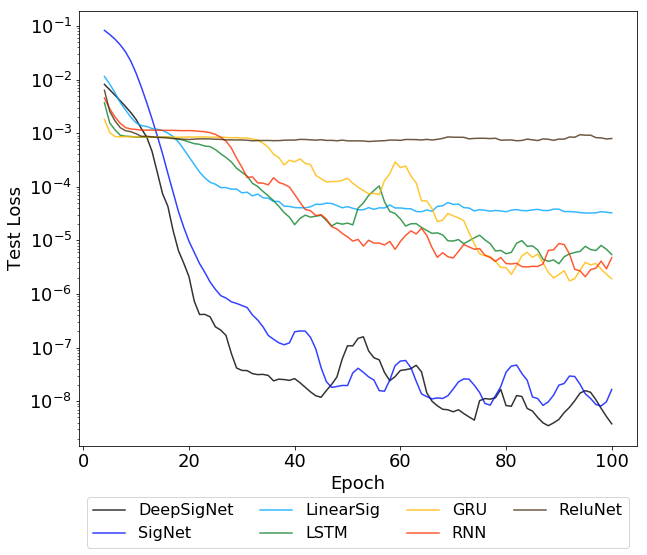
\includegraphics[width=\linewidth]{figures/final_results}
			\caption{Test loss by epoch}
	\end{subfigure}
	\begin{subfigure}{0.5\textwidth}
			\centering
			\begin{tabular}{l c c} \toprule
			    {} & {Test Loss} & {\# Params} \\ \midrule
			    $\text{Rescaled Range}$ & 0.0032 & N/A \\
			    $\text{Feedforward}$ & 0.0471 & 11889 \\
			    $\text{RNN}$  & 0.0088 & 10635  \\	
			    $\text{GRU}$  & 0.0047  & 9780   \\
			    $\text{LSTM}$  & 0.0039 & 10832  \\
			    $\text{Linear-Sig}$  & 0.0112 & 10313 \\
			    $\text{SigNet}$  & 0.0009 & 8777  \\
			    $\text{DeepSigNet}$  & \textbf{0.0002} & 9741  \\ \bottomrule
			\end{tabular}
			\caption{Final test loss}
	\end{subfigure}
	\caption{Performance at estimating the Hurst parameter for various models with and without signatures.}
	\label{fig:fbm results}
\end{figure}

All models were trained for the same number of epochs using the Adam \cite{TODO} optimiser as implemented by PyTorch \cite{TODO}, which was the framework used to implement the models. Also shown are the results of the rescaled range method \cite{TODO}. The data was also flattened and fed into a non-recurrent feedforward model, referred to as Feedforward, as a baseline in the context of neural networks, whilst the na{\"i}ve Linear-Sig model outlined previously in Figure \ref{fig:linear-sig} provides a baseline from the context of signatures. SigNet and DeepSigNet are both models of the sort described by Figure \ref{fig:deep signatures}; SigNet has a single Neural-Lift-Signature block, whilst DeepSigNet has two. \TODO[Say a little more about the architectures. (size activation etc.)\\]

 % TODO: ReluNet -> Feedforward in two places
 % TODO: scientific notation

\begin{figure}
\centering
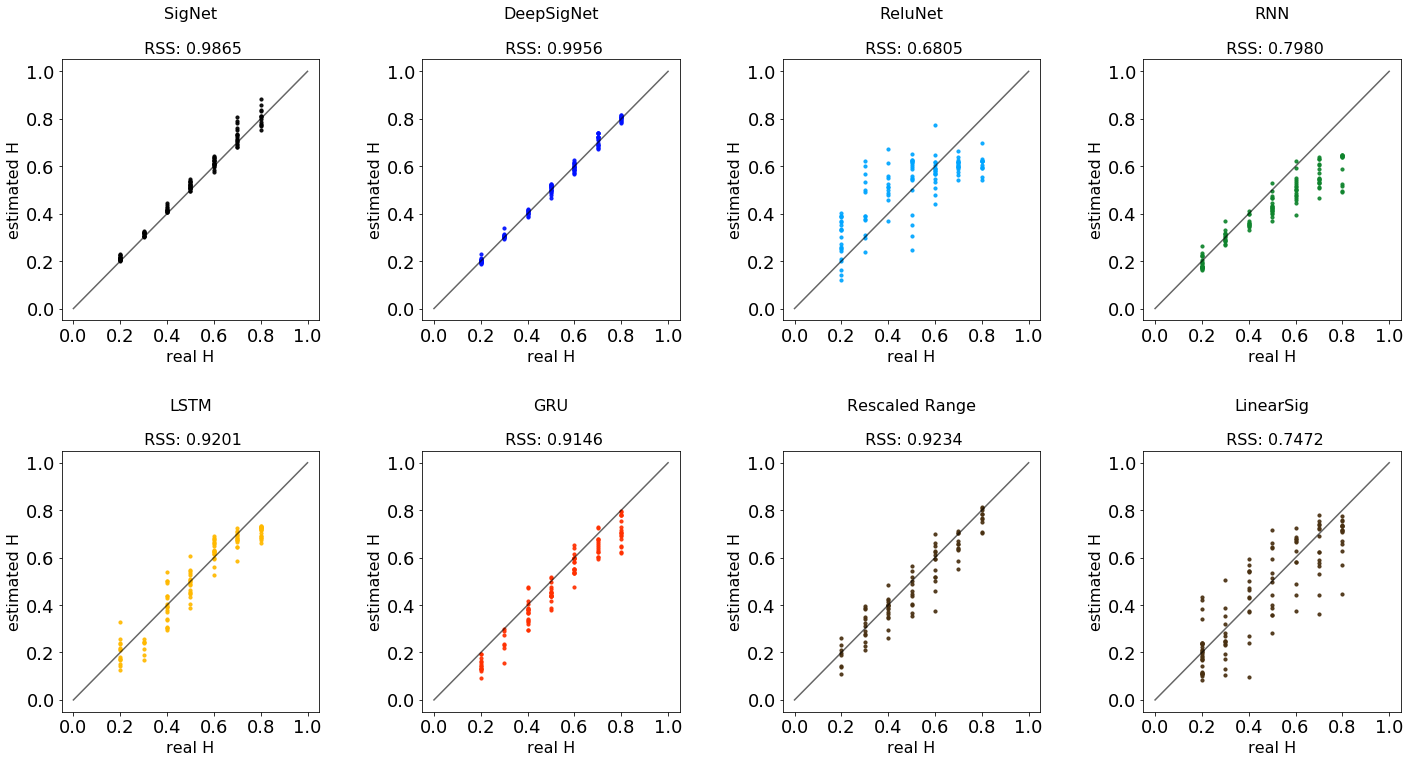
\includegraphics[width=\textwidth]{figures/hurst_est}
\caption{Real vs predicted Hurst parameters.}
\label{fig:fbm comparison}
\end{figure}
\section{Inverting the truncated signature}\label{subsec:inverting signature}

Given a truncated signature, we might seek to recover the original stream of data. The signature map is essentially injective (up to tree-like equivalence, see Appendix \ref{appendix:sigprop}), so this is a well-posed problem in principle. One immediate hurdle is that in practice we have the truncated signature rather than the full signature. Even given the full signature, finding a mathematical description of the inversion is a challenging task \cite{lyons2014inverting, chang2017signature, chang2018effective}.

In this experiment we show how the signature layer can be used to perform this task. Fix a stream of data $\mathbf x = (x_1, \ldots, x_n) \in \mathcal S(\mathbb R^d)$. Assume that the truncated signature $\mathrm{Sig}^N(\mathbf x)$ and the number of steps $n\in \mathbb N$ are known; we seek to reconstruct the stream of data $\mathbf x$. The strategy now is to minimise the following loss function, using backpropagation:
\begin{equation*}
L(\mathbf y; \mathbf x) = \frac{1}{2} \left \lVert \mathrm{Sig}^N(\mathbf y) - \mathrm{Sig}^N(\mathbf x)\right \rVert_2^2\quad \mbox{for }\mathbf y=(y_1, \ldots, y_n)\in \mathcal S(\mathbb R^d).
\end{equation*}
%If one wishes this may be described by a simple neural network.

Figure \ref{fig:invertedsig} shows four handwritten digits from the PenDigits dataset \cite{UCI}, for which $n=\TODO$. The solid blue path is the original path $\mathbf x$, whilst the dashed orange path is the reconstructed path $\mathbf y$ minimising $L(\mathbf y; \mathbf x)$. Truncated signatures of order $N=12$ were used for this task. We see that the truncated signatures have managed to encode the input paths $\mathbf x$ almost perfectly.

\begin{figure}
\centering
\begin{minipage}{.2\textwidth}
  \centering
  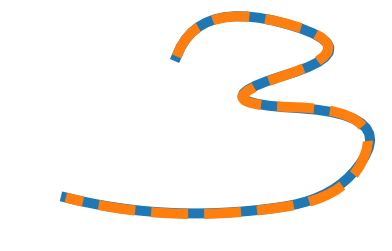
\includegraphics[width=0.9\linewidth]{figures/3}
\end{minipage}
\begin{minipage}{.2\textwidth}
  \centering
  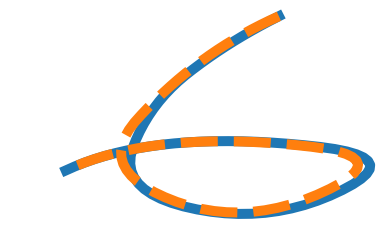
\includegraphics[width=0.9\linewidth]{figures/6}
\end{minipage}
\begin{minipage}{.2\textwidth}
  \centering
  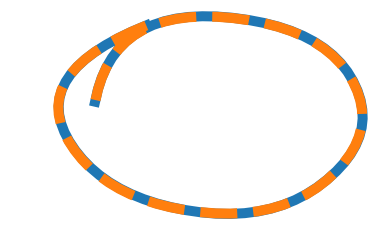
\includegraphics[width=0.9\linewidth]{figures/0}
\end{minipage}
\begin{minipage}{.2\textwidth}
  \centering
  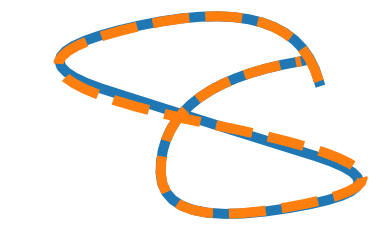
\includegraphics[width=0.9\linewidth]{figures/8}
\end{minipage}%
\caption{Original path (blue) and path reconstructed from its signature (dashed orange) for four handwritten digits in the PenDigits dataset \cite{UCI}.}
\label{fig:invertedsig}
\end{figure}

\section{A generative model for a stochastic process}

\newcommand{\offset}{-0.5}
\begin{figure}[t]
	\centering
	\resizebox{\textwidth}{!}{%
		\begin{tikzpicture}
		%Brownian motion
		\node (Position) at (0,0) {};
			%box
			\draw[black, fill=green!30, thick] (Position) rectangle ++(1,2);	%Body
			%Annotations brackets
			\draw ($ (Position) + (-.2,0) $) -- ++(-0.2,0) -- ++(0,2) -- ++(0.2,0); %left
			\draw ($ (Position) + (0,-0.2) $) -- ++(0,-.2) -- ++(1,0) -- ++(0,.2); %bottom
			%Annotations
			\node[align=center,font=\large](centre) at ($ (Position) + (.5,1) $){$ B_t $}; %centre
			\node[align=center,font=\small, rotate=90](left) at ($ (Position) + (-.53,0.5) $){Steps}; %left
			\node[align=center,font=\small](bottom) at ($ (Position) + (.5,-0.6) $){Channels}; %bottom
			%Arrow
			\draw[->] ($ (Position) + (1.25,1) $) -- ++(1 + \offset,0);
		
		%Augmentation
		\node (Position) at (2.75 + \offset,0) {};
			%box
			\draw[black, fill=blue!30, thick] (Position) rectangle ++(1,2);	%Body
			%Annotations brackets
			\draw ($ (Position) + (-.2,0) $) -- ++(-0.2,0) -- ++(0,2) -- ++(0.2,0); %left
			\draw ($ (Position) + (0,-0.2) $) -- ++(0,-.2) -- ++(1,0) -- ++(0,.2); %bottom
			%Annotations
			\node[align=center,font=\large](centre) at ($ (Position) + (.5,1) $){$ \Phi $}; %centre
			\node[align=center,font=\small, rotate=90](left) at ($ (Position) + (-.53,0.5) $){Steps}; %left
			\node[align=center,font=\small](bottom) at ($ (Position) + (.5,-0.6) $){Channels}; %bottom
			%Arrow
			\draw[->] ($ (Position) + (1.25,1) $) -- ++(1 + \offset,0);
		
		%Lift
		\node (Position) at (5.5 + 2 * \offset,0) {};
			%box
			\draw[black, fill=blue!30, thick] (Position) rectangle ++(1,2);	%Body
			\draw[fill=blue!20, thick]  ($ (Position) + (0,2) $) -- ++(.5,.5) -- ++(1,0) -- ++(-.5,-.5) -- cycle; %top
			\draw[fill=blue!70!black!40, thick]  ($ (Position) + (1,0) $) -- ++(.5,.5) -- ++(0,2) -- ++(-.5,-.5) -- cycle; %side	
			%Annotations brackets
			\draw ($ (Position) + (-.2,0) $) -- ++(-0.2,0) -- ++(0,2) -- ++(0.2,0); %left
			\draw ($ (Position) + (0,-0.2) $) -- ++(0,-.2) -- ++(1,0) -- ++(0,.2); %bottom
			\draw ($ (Position) + (-.2,2.2) $) -- ++(-.2,.2) -- ++(.5,.5) -- ++(.2,-.2); %top
			%Annotations
			\node[align=center, font=\large](centre) at ($ (Position) + (.5,1) $){ $\ell$ }; %centre
			\node[align=center,font=\small, rotate=90](left) at ($ (Position) + (-.53,0.5) $){Steps}; %left
			\node[align=center,font=\small](bottom) at ($ (Position) + (.5,-0.6) $){Channels}; %bottom
			\node[align=center,font=\small, rotate=45](top) at ($ (Position) + (-.35,2.8) $){Steps of steps}; %top
			%Arrow
			\draw[->] ($ (Position) + (1.25,1) $) -- ++(1 + \offset,0);
		
		%Sig
		\node (Position) at (8.25 + 3 * \offset ,0) {};
			%box
			\draw[black, fill=blue!30, thick] (Position) rectangle ++(1,2);	%Body
			%Annotations brackets
			\draw ($ (Position) + (-.2,0) $) -- ++(-0.2,0) -- ++(0,2) -- ++(0.2,0); %left
			\draw ($ (Position) + (0,-0.2) $) -- ++(0,-.2) -- ++(1,0) -- ++(0,.2); %bottom
			%Annotations
			\node[align=center](centre) at ($ (Position) + (.5,1) $){$ \mathrm{Sig}^N $}; %centre
			\node[align=center,font=\small, rotate=90](left) at ($ (Position) + (-.53,0.5) $){Steps}; %left
			\node[align=center,font=\small](bottom) at ($ (Position) + (.5,-0.8) $){Signature \\ terms}; %bottom
			%Arrow
			\draw[->] ($ (Position) + (1.25,1) $) -- ++(1 + \offset,0);
		
		%Linear
		\node (Position) at (11 + 4 * \offset,0) {};
			%box
			\draw[black, fill=blue!30, thick] (Position) rectangle ++(1,2);	%Body
			%Annotations brackets
			\draw ($ (Position) + (-.2,0) $) -- ++(-0.2,0) -- ++(0,2) -- ++(0.2,0); %left
			\draw ($ (Position) + (0,-0.2) $) -- ++(0,-.2) -- ++(1,0) -- ++(0,.2); %bottom
			%Annotations
			\node[align=center,font=\large](centre) at ($ (Position) + (.5,1) $){$ L $}; %centre
			\node[align=center,font=\small, rotate=90](left) at ($ (Position) + (-.53,0.5) $){Steps}; %left
			\node[align=center,font=\small](bottom) at ($ (Position) + (.5,-0.6) $){Channels}; %bottom
			%Arrow slanted
			\draw[->] ($ (Position) + (1.25,1) $) -- ++(1 + \offset,0);
		

		% Sig 2, sample and text		
		\node (Position) at (13.75 + 5 * \offset, 0) {};
			%box
			\draw[black, fill=blue!30, thick] (Position) rectangle ++(1,2);	%Body
			%Annotations brackets
			\draw ($ (Position) + (-.2,0) $) -- ++(-0.2,0) -- ++(0,2) -- ++(0.2,0); %left
			\draw ($ (Position) + (0,-0.2) $) -- ++(0,-.2) -- ++(1,0) -- ++(0,.2); %bottom
			%Annotations
			\node[align=center](centre) at ($ (Position) + (.5,1) $){$ \mathrm{Sig}^M $}; %centre
			\node[align=center,font=\small, rotate=90](left) at ($ (Position) + (-.53,0.5) $){Steps}; %left
			\node[align=center,font=\small](bottom) at ($ (Position) + (.5,-0.8) $){Signature \\ terms}; %bottom
			%Arrow
			\draw[->] ($ (Position) + (1.25,1) $) -- ++(1 + \offset,0) -- ++(.8,-.8);
			
			
			%Separating line
			\draw[densely dotted] ($ (Position) + (5,2.5) $) -- ++(-5.75,0) -- ++(0,-3.7) -- ++(-7.15,0) -- ++(0,-2.9);
			%Gan text
			\node[align=center, font=\large](left) at ($ (Position) + (-7.75 - 1.8,-2.5) $){Generator}; 
			%Desc text
			\node[align=center, font=\large](left) at ($ (Position) + (-7.75 + 1.8,-2.5) $){Discriminator};
			%Test
			\draw[fill=red!40, thick] ($ (Position) + (3.8 + \offset,-0.8) $) circle (1);
			\node[align=center](centre) at ($ (Position) + (3.8 + \offset,-0.9) $){Two-sample \\ test}; 			
		
		%Sample path
		\node (Position) at (11 + 4 * \offset,-3.5) {};
			%box
			\draw[black, fill=green!30, thick] (Position) rectangle ++(1,2);	%Body
			%Annotations brackets
			\draw ($ (Position) + (-.2,0) $) -- ++(-0.2,0) -- ++(0,2) -- ++(0.2,0); %left
			\draw ($ (Position) + (0,-0.2) $) -- ++(0,-.2) -- ++(1,0) -- ++(0,.2); %bottom
			%Annotations
			\node[align=center,font=\large](centre) at ($ (Position) + (.5,1) $){$ X_t $}; %centre
			\node[align=center,font=\small, rotate=90](left) at ($ (Position) + (-.53,0.5) $){Steps}; %left
			\node[align=center,font=\small](bottom) at ($ (Position) + (.5,-0.6) $){Channels}; %bottom
			%Arrow
			\draw[->] ($ (Position) + (1.25,1) $) -- ++(1 + \offset,0);
		
		%Sig 3
		\node (Position) at (13.75 + 5 * \offset,-3.5) {};
			%box
			\draw[black, fill=blue!30, thick] (Position) rectangle ++(1,2);	%Body
			%Annotations brackets
			\draw ($ (Position) + (-.2,0) $) -- ++(-0.2,0) -- ++(0,2) -- ++(0.2,0); %left
			\draw ($ (Position) + (0,-0.2) $) -- ++(0,-.2) -- ++(1,0) -- ++(0,.2); %bottom
			%Annotations
			\node[align=center](centre) at ($ (Position) + (.5,1) $){$ \mathrm{Sig}^M $}; %centre
			\node[align=center,font=\small, rotate=90](left) at ($ (Position) + (-.53,0.5) $){Steps}; %left
			\node[align=center,font=\small](bottom) at ($ (Position) + (.5,-0.8) $){Signature \\ terms}; %bottom
			%Arrow
			\draw[->] ($ (Position) + (1.25,1) $) -- ++(1 + \offset,0) -- ++(.8,.8);
		
		
		\end{tikzpicture}
	}
	\caption{Generative model architecture}
	\label{GAN-arch}	
\end{figure}

 % TODO: get legend outside of the plot
\begin{wrapfigure}{r}{0pt}
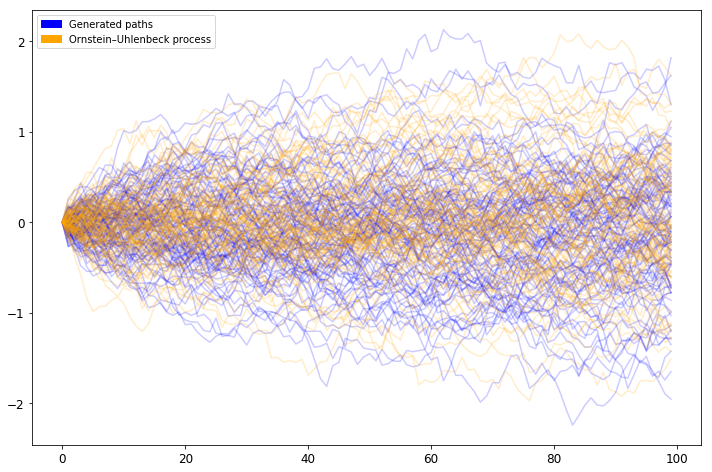
\includegraphics[width=0.5\textwidth]{figures/OU}
\captionsetup{width=0.9\linewidth}
\caption{Generated paths alongside the original paths.}
\label{fig:OU}
\end{wrapfigure}

Generative models are typically trained to learn to transform random noise to a target distribution. One common approach are Generative Adversarial Networks (GANs) \cite{goodfellow2014generative}. An alternative approach is to define a distance on the space of distributions by embedding them into a Reproducing Kernel Hilbert Space (RKHS). The discriminator is then a fixed two-sample test based on a kernel maximum mean discrepancy \cite{gmmn2015, traininggmmns2015, gretton2017}. This is known as a Generative Moment Matching Network (GMMN).

With this framework we propose a signature-based generative model for sequential data.

Following \cite{kiraly2016kernels, chevyrev2018signature}, the kernel $k$ is given by
\[ k \colon \mathcal S(\mathbb R^d) \times \mathcal S(\mathbb R^d) \to \mathbb R, \quad k(\mathbf{x},\mathbf{y}) = \left (\mathrm{Sig}^N \left (\lambda_{\mathbf{x}} \mathbf x\right ), \mathrm{Sig}^N\left (\lambda_{\mathbf{y}}\mathbf y\right ) \right ), \]
where $\lambda_{\mathbf x}\in \mathbb R$ is a certain normalising constant guaranteeing that $k$ is the kernel of a RKHS and $(\,\cdot\, , \,\cdot\,)$ denotes the dot product. Then given $m$ samples $\{\mathbf y^{(i)}\}_{i=1}^n \subseteq \mathcal S(\mathbb R^d)$ from the target distribution and $n$ samples $\{\mathbf x^{(i)}\}_{i=1}^n \subseteq \mathcal S(\mathbb R^d)$ from the generator, the loss is given by
\[T\left (\{\mathbf x^{(i)}\}_{i=1}^n, \{\mathbf y^{(i)}\}_{i=1}^m\right ) = \dfrac{1}{n^2}\sum_{i, j} k(\mathbf{x}^{(i)},\mathbf{x}^{(j)}) - \dfrac{2}{nm}\sum_{i, j} k(\mathbf{x}^{(i)},\mathbf{y}^{(j)}) + \dfrac{1}{m^2}\sum_{i, j} k(\mathbf{y}^{(i)},\mathbf{y}^{(j)}).\]

The proposed model is shown in Figure \ref{GAN-arch}; there is an implicit batch dimension throughout. The input to the network is Brownian motion $B_t$. This is fed through a small neural network $\Phi$ and lifted to a stream of streams by $\ell$. The truncated signature is then applied stream-wise, and finally a linear layer is placed on the end. In a nice twist, both the generator and the discriminator involve the signature. Observe how the generative part is a particular case of the general form proposed in Figure \ref{fig:deep signatures}.

We applied the proposed generative model to a dataset of 1024 realisations of an Ornstein--Uhlenbeck process \cite{uhlenbeck1930theory}. The layer $\Phi$ was taken to be a small neural network with 2 output neurons and one hidden layer of 8 neurons, and a ReLU activation function, operating pointwise on the stream $(\mathbf{B_t},\mathbf{t}) \in S(\mathbb R^2)$. The signature was truncated at $N=3$ and linearly mapped by $L$ down to dimension 2. Figure \ref{fig:OU} shows the generated paths alongside the original ones. Minimising the loss function $T$ implies that the generated paths are almost indistinguishable from the real Ornstein--Uhlenbeck process.

\section{Reinforcement Learning}
	
	\subsubsection*{Acknowledgements}
	PK was supported by the Engineering and Physical Sciences Research Council [EP/L015811/1]. \TODO[Any other acknowledgements.]
	
	\TODO[Tidy up bibliography: there's quite a lot of `arXiv preprint arXiv']
	
	\small
	\bibliography{references} 
	\bibliographystyle{ieeetr}
	
	\normalsize
	\newpage % Need to start it on a new page so we can submit appendices separately, I think
	\appendix
\section{A brief overview of signatures}\label{appendix:sigprop} 
\subsection{Properties of signatures}
\begin{definition}[\cite{lyons1998differential}] 
	Let $a, b \in \mathbb R$, and $X = (X^1, \ldots, X^d) \colon [a, b] \to \mathbb R^d$ be a continuous piecewise smooth path.  The signature of $X$ is then defined as the collection of iterated integrals
	\begin{align*}
	\mathrm{Sig}(X) &= \left( \int_{a < t_1 < \cdots < t_k < b} \mathrm dX_{t_1} \otimes \cdots \otimes  \mathrm dX_{t_k} \right)_{k \geq 0}\\
	&= \left(\left( \int_{a < t_1 < \cdots < t_k < b} \mathrm dX^{i_1}_{t_1} \cdots \mathrm dX^{i_k}_{t_k} \right)_{1 \leq i_1, \ldots, i_k \leq d}\right)_{k\geq 0},
	\end{align*}
	where $\otimes$ denotes the outer product, $  \mathrm dX_t = \frac{\mathrm dX_t}{\mathrm dt}{\mathrm dt} $, and the $k = 0$ term is taken to be $1 \in \mathbb R$.
	
	The (truncated) signature of order $N$ of $X$ is defined as
	\begin{equation*}
	\mathrm{Sig}^N(X)= \left( \int_{a < t_1 < \cdots < t_k < b} \mathrm dX_{t_1} \otimes \cdots \otimes  \mathrm dX_{t_k} \right)_{0 \leq k \leq N}.
	\end{equation*}
\end{definition}
The signature may in fact be defined much more generally, on paths of merely bounded variation, see \cite{lyons1998differential, FritzVictoir10}, but the above definition suffices for our purposes. This broader theory is also the reason behind the notation $\mathrm dX_t$, which may be made sense of even when $X$ is not continuous or differentiable.

\begin{example} \label{ex:sigincrement}
	Suppose $X \colon [a, b] \to \mathbb R^d$ is the linear interpolation of two points $ x,y \in \mathbb R^d $, so that $ X_t = x + \frac{t-a}{b-a}(y-x) $ . Then its signature is just the collection of powers of its total increment:
	\begin{equation*}
	\mathrm{Sig}(X) = \left(1, y-x, \frac{1}{2} (y-x)^{\otimes 2}, \frac{1}{6} (y-x)^{\otimes 3}, \ldots, \frac{1}{k!} (y-x)^{\otimes k}, \ldots \right).
	\end{equation*}
	Which is independent of $a$, $b$.
\end{example}

%\begin{example}
%Suppose $X \colon [0, 1] \to \mathbb R$, so that the dimension of the codomain is one. Then its signature is just the collection of powers of its total increment:
%\begin{equation*}
%\mathrm{Sig}(X) = \left(X_1 - X_0, \frac{1}{2} (X_1 - X_0)^2, \frac{1}{6} (X_1 - X_0)^3, \ldots, \frac{1}{n!} (X_1 - X_0)^n, \ldots \right)
%\end{equation*}
%\end{example}

% Signatures of paths were first studied by Chen \cite{Chen54, Chen57, Chen58}, who showed that it determines any piecewise affine path up to 'tree-like equivalence' and that nonlinear functions on the signature can be expressed as linear functions on the coordinates. More recently they have been studied in the context of rough path theory as a way of describing the solution to differential equations when the input signal has very low regularity. See \cite{lyons1998differential, FritzVictoir10} for more on this

The signature exhibits three key properties that makes their use attractive when dealing with path-like data. First, a path is essentially defined by its signature. This means that essentially no information is lost when applying the signature map.% The following is an extension of Chens original result mentioned above:
\begin{proposition}[Uniqueness of signature \cite{hambly2010uniqueness}]\label{prop:uniqueness}
	Let $X \colon [a, b] \to \mathbb R^d$ be a continuous piecewise smooth path. Then $\mathrm{Sig}(X)$ uniquely determines $X$ up to `tree-like equivalence'.
\end{proposition}

Next, the terms of the signature decay in size factorially. This means that little information is lost when truncating the signature.
\begin{proposition}[{Factorial decay \cite[Lemma 2.1.1]{lyons1998differential}}]
	Let $X \colon [a,b]\to \mathbb R^d$ be a continuous piecewise smooth path. Then
	\begin{equation*}
	\left \lVert \int_{a < t_1 < \cdots < t_n < b} dX_{t_1} \otimes \cdots \otimes  dX_{t_n} \right \rVert \leq \dfrac{C(X)^N}{N!},
	\end{equation*} 
	where $C(X)$ is a constant depending on $X$ and $ \lVert \,\cdot\, \rVert $ is any tensor norm on $ (\mathbb R^d)^{\otimes n} $.
\end{proposition}

Finally, functions of the path are approximately linear on the signature. In some sense the signature may be thought of as a `universal nonlinearity' on paths.
\begin{proposition}[Universal approximation theorem for signatures \cite{lyons2014rough}]\label{prop:universal}
	Let $F$ be a real-valued continuous function on continuous piecewise smooth paths and let $\mathcal K $ be a compact set of such paths.\footnote{Of course the definition of both continuity and compactness depend on the topology of the set of paths. See \cite{lyons2014rough} for details.} Let $\varepsilon >0$. Then there exists a linear functional $L$ such that
	\begin{equation*}\left \vert F(X) - L(\mathrm{Sig}(X)) \right\vert < \varepsilon \quad \forall \, X \in \mathcal K.
	\end{equation*}
\end{proposition}

\subsection{Computing signatures}
The signature is little more than a mathematical idealisation unless we can compute it. Fortunately, this is possible, and in an efficient manner too.

Observe that the signature of a path $ X \colon [a,b] \to \mathbb R^d $ can be described as a sequence where the zeroth term is $1 \in (\mathbb {R}^d)^{\otimes 0} = \mathbb {R} $, the first term belongs to $\mathbb {R}^d$, the second term belongs to $ \mathbb {R}^d \otimes \mathbb {R}^d $, and the $k$th term belongs to $(\mathbb {R}^d)^{\otimes k} = \mathbb {R}^d \otimes \cdots \otimes \mathbb {R}^d$, $ k $ times. With this description, the signature of a path naturally takes values in the tensor algebra:
\begin{definition}
	The tensor algebra of $\mathbb R^d$ is defined as
	\begin{equation*}
	T((\mathbb R^d)) = \prod_{k = 0}^\infty (\mathbb {R}^d)^{\otimes k}.
	\end{equation*}
	The tensor product, when extended by bilinearity, naturally defines a multiplication on $ T((\mathbb R^d)) $. For $A = (A_0, A_1, \ldots) \in T((\mathbb R^d))$ and $B = (B_0, B_1, \ldots) \in T((\mathbb R^d))$, then $A \otimes B \in T((\mathbb R^d))$ can be seen to be
	\begin{equation*}
	A \otimes B = \left(\sum_{j = 0}^k A_j \otimes B_{k - j}\right)_{k \geq 0}.
	\end{equation*}
\end{definition}

A fundamental insight of Chen is that concatenation of paths corresponds to multiplication of their signatures. The following relation is known as \textit{Chen's identity}.
\begin{proposition}[{Chen's identity, \cite[Theorem 2.12]{lyons1998differential}}]
	Let $X \colon [a,b] \to \mathbb R^d$ and $Y \colon [a,b] \to \mathbb R^d$ be two continuous piecewise smooth paths such that $X_b = Y_a$. Define their concatenation $X\ast Y$ as
	\begin{empheq}[left={(X\ast Y)_t = \empheqlbrace}]{align*}
	X_{2t-a} &\quad\text{for}\quad a \leq t < \frac{a+b}{2},\\
	Y_{2t -b}  &\quad\text{for}\quad \frac{a+b}{2} \leq t \leq b.
	\end{empheq}
	Then
	\begin{equation*}
	\mathrm{Sig}(X\ast Y) = \mathrm{Sig}(X) \otimes \mathrm{Sig}(Y).
	\end{equation*}
\end{proposition}

Everything so far has operated on paths. In practice, of course, one has some stream of data, which we interpret as a discretisation of a path.
\begin{definition}
	The space of streams of data is defined as
	\begin{equation*}
	\mathcal S(\mathbb R^d) = \{ \mathbf x=(x_1, \ldots, x_n) : x_i \in \mathbb R^d, n \in \mathbb N\}.
	\end{equation*}
	Given $\mathbf x=(x_1, \ldots, x_n) \in \mathcal S(\mathbb R^d)$, the integer $n$ is called the length of $\mathbf x$. Furthermore for $ a , b \in \mathbb R $ such that $ a < b $, fix
	\begin{equation*}
	a = u_1 < u_2 < \cdots < u_{n - 1} < u_n = b.
	\end{equation*}
	Let $X = (X^1, \ldots, X^d) \colon [a,b] \to \mathbb R^d$ be continuous such that $X_{u_i} = x_i$ for all $i$, and linear on the intervals in between. Then $X$ is called a linear interpolation of $\mathbf x$.
\end{definition}

\begin{definition}\label{def:sig}
	Let $\mathbf x=(x_1, \ldots, x_n)\in \mathcal S(\mathbb R^d)$ be a stream of data. Let $X$ be a linear interpolation of $\mathbf x$. Then the signature of $\mathbf x$ is defined as
	\begin{equation*}
	\mathrm{Sig}(\mathbf x) = \mathrm{Sig}(X)
	\end{equation*}
	and the (truncated) signature of order $N$ of $\mathbf x$ is defined as
	\begin{equation*}
	\mathrm{Sig}^N(\mathbf x) = \mathrm{Sig}^N(X).
	\end{equation*}
\end{definition}
\emph{A priori} this definition of the signature of a stream of data depends on the choice of linear interpolation. However, it turns out that Definition \ref{def:sig} is well-defined and independent of this choice, see \cite[Lemma 2.12]{lyons1998differential}.

\begin{remark}
	Let $\mathbf x = (x_1, \ldots, x_n) \in \mathcal S(\mathbb R^d)$ be a stream of data of length $n$ in $ \mathbb{R}^d $. Then $\mathrm{Sig}^N(\mathbf x)$ has
	\begin{equation*}
	\sum_{k = 0}^N d^k = \frac{d^{N+1} - 1}{d-1}
	\end{equation*}
	components. In particular, the number of components does not depend on $n$; the truncated signature maps the infinite-dimensional space of streams of data $\mathcal S(\mathbb R^d)$ into a finite-dimensional space of dimension $(d^{N+1} - 1)/(d-1)$. Thus the signature is an excellent way to tackle long streams of data, or streams of variable length.
\end{remark}

Equipped with Chen's identity, the signature of a stream is straightforward to compute explicitly.
\begin{proposition}
	Let $\mathbf x = (x_1, \ldots, x_n)\in \mathcal S(\mathbb R^d)$ be a stream of data. Then,
	\begin{equation*}
	\mathrm{Sig}(\mathbf x) = \exp(x_2 - x_1) \otimes \exp(x_3 - x_2) \otimes \cdots \otimes \exp(x_n - x_{n-1}),
	\end{equation*}
	where
	\[\exp(x) = \left(\frac{x^{\otimes k}}{k!}\right)_{k \geq 0}.\]
\end{proposition}
\begin{proof}
	It is easy to check that if $\mathbf x = (x_1, x_2)\in \mathcal S(\mathbb R^d)$ is a stream of data of length 2 then the signature of $\mathbf x$ is given by $\exp(x_2 - x_1)$, as in Example \ref{ex:sigincrement}. So given a stream of data $\mathbf x = (x_1, \ldots, x_n)\in \mathcal S(\mathbb R^d)$ of length $n \geq 2$, iteratively applying Chen's identity yields the result.
\end{proof}

\begin{remark} \label{re:efficiency}
	Chen's identity implies that computing the signature of an incoming stream of data is efficient. Indeed, suppose one has obtained a stream of data $\mathbf x\in \mathcal S(\mathbb R^d)$ and computed its signature. Suppose that after some time more data has arrived, $\mathbf y \in \mathcal S(\mathbb R^d)$. In order to compute the signature of the whole signal one only needs to compute the signature of the new piece of information, and tensor product it with the already-computed signature.
\end{remark}

\begin{remark}
	The signature has one final property, which we have actually already briefly touched upon, which is that it is invariant to reparameterisations. Formally speaking, if $X \colon [0, 1] \to \mathbb R^d$ is a continuous path, and $\psi \colon [0, 1] \to [0, 1]$ is an orientation-preserving diffeomorphism, then $\mathrm{Sig}(X) = \mathrm{Sig}(X \circ \psi)$. It is the reason why the signature of a stream of data is invariant to the choice of linear interpolation. Thus the signature encodes the \emph{order} in which data arrives without caring precisely \emph{when} it arrives. For example, consider the scenario of recording the movement of a pen as it draws a character on a piece of paper. Then the signature of the stream of data is invariant to the speed at which the character was drawn.
\end{remark}
\end{document}